\documentclass[12pt]{article} \setlength{\oddsidemargin}{0in}
\setlength{\evensidemargin}{0in} \setlength{\textwidth}{6.5in}
\setlength{\parindent}{0in} \setlength{\textwidth}{16cm}
\setlength{\topmargin}{1in} \addtolength{\topmargin}{-1.5in}
\setlength{\textheight}{23cm} \setlength{\parskip}{0.75cm}

% Brackets
\usepackage{mathtools} \DeclarePairedDelimiter\ceil{\lceil}{\rceil}
\DeclarePairedDelimiter\floor{\lfloor}{\rfloor}

% Tikz settings
\usepackage{tikz} \usetikzlibrary{trees} \usetikzlibrary {positioning}
\definecolor {mypurple}{cmyk}{0.6,0.4,0.1,0} \definecolor
{myred}{cmyk}{0,0.3,0.3,0} \usetikzlibrary{fit,shapes.misc}

% Typesetting options
\usepackage{fancyvrb} \usepackage{amsmath,amsfonts,amssymb}
\usepackage [english]{babel} \usepackage [autostyle, english =
american]{csquotes} \usepackage[none]{hyphenat} \usepackage{url}

\begin{document}

\noindent CSCI 3104 Spring 2018 \hfill Problem Set 8\\
Cole Schlisner (3/22)

% Image
\graphicspath{ {images/} }

\hrulefill

{\fontfamily{cmr}\selectfont}

% ******************* PROBLEM 1 *********************
\section*{Problem 1}

\textit{(10 pts) Ginerva Weasley is playing with the network given
  below. Help her calculate the number of paths from node 1 to node
  14.}

\textit{Hint: assume a ``path'' must have at least one edge in it to
  be well defined, and use dynamic programming to fill in a table that
  counts number of paths from each node j to 14, starting from 14 down
  to 1.}


\begin{figure}[h]
  \centering 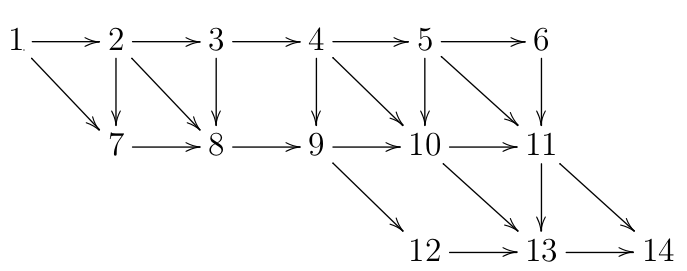
\includegraphics[width=0.8\textwidth]{P1}
\end{figure}

There are 30 paths from node 1 to to node 14. 
This was calculated by filling in the following table:


\begin{tabular}{ |p{1cm}||p{.5cm}|p{.5cm}|p{.5cm}|p{.5cm}|p{.5cm}|p{.5cm}|p{.5cm}|p{.5cm}|p{.5cm}|p{.5cm}|p{.5cm}|p{.5cm}|p{.5cm}|p{.5cm}| }
 \hline
  j &14&13&12&11&10&9&8&7&6&5&4&3&2&1   \\
 \hline
 \hline
  $X_{j,14}$ &0&1&1&2&3&4&4&4&2&7&14&18&26&30 \\
 \hline
\end{tabular}

The above table was filled in from left to right. Starting at j=14: there are 0 paths from 14 to 14 because as the problem states, a path must have at least one edge in it to be well defined. The base cases in this dynamic programming table are the nodes 13 and 11, as they are immediate neighbors to 14. Every subsequent node can be calculated using the nodes already filled in. For example - 12 (the second node to be filled in) only has a path to node 13, which itself has 1 path to 14 thus there is only 1 path from 12 to 14. Similarly, there is a path from node 5 to nodes 6, 11, and 10 which each have 2, 2, and 3 paths to 14 respectively. This means there are 2 + 2 + 3 = 7 paths from node 5 to node 14. Applying this logic for every node allows every path to 14 to be implicitly enumerated. 

\newpage

% ******************* PROBLEM 2 *********************
\section*{Problem 2}

\textit{(10 pts) Ginny Weasley needs your help with her wizardly
  homework. She’s trying to come up with an example of a directed
  graph $G = (V, E)$, a start vertex $s \in V$ and a set of tree edges
  $E_T \subseteq E$ such that for each vertex $v \in V$, the unique path in the
  graph $(V, E_T)$ from $s$ to $v$ is a shortest path in $G$, yet the
  set of edges $E_T$ cannot be produced by running a depth-first
  search on $G$, no matter how the vertices are ordered in each
  adjacency list. Include an explanation of why your example satisfies
  the requirements.} \\\\
Consider the following graph G, set of tree edges $E_T$, and starting vertex $s$:\\
  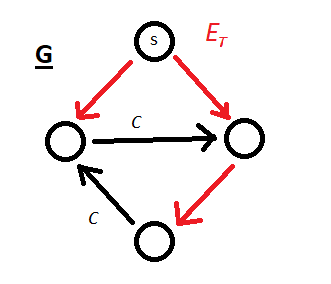
\includegraphics[width=6cm,height=6cm]{2-G-ET}

  There are only 2 different paths that DFS could take from $s$ to explore the entire graph.
  Here are visualizations of these paths using the notation for timestamps (d/f) from CLRS.

  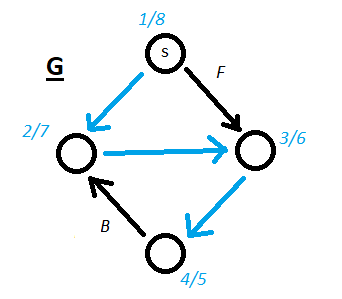
\includegraphics[width=6cm,height=6cm]{2-G-P1} 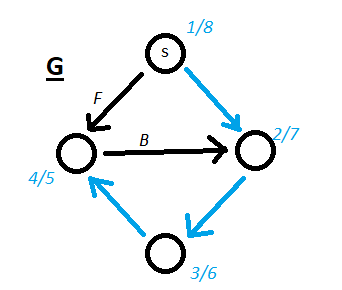
\includegraphics[width=6cm,height=6cm]{2-G-P2} 

  Both paths leave out one of the edges in $E_T$. 

\newpage

% ******************* PROBLEM 3 *********************
\section*{Problem 3}

\textit{(15 pts) Prof. Dumbledore needs your help to compute the in-
  and out-degrees of all vertices in a directed multigraph
  $G$. However, he is not sure how to represent the graph so that the
  calculation is most efficient. For each of the three possible
  representations, express your answers in asymptotic notation (the
  only notation Dumbledore understands), in terms of $V$ and $E$, and
  justify your claim.}

\begin{enumerate}
\item[(a)]{\textit{An \textbf{adjacency matrix} representation. Assume
      the size of the matrix is known.}}\\\\
  $\Theta(|V|^2)$ - In order to calculate the degree of all nodes, you would need to visit each row of the matrix m[i][*], and scan across all of the entries (m[i][j]) in order to read the number of incoming and outgoing edges between V[i] and V[j]. Assuming this information is already stored in the entries in m, reading the data is a constant time operation.\footnote{If $m[i][j] = (\sum{[1 \forall (V_i,V_j) \in E]} , \sum{[1 \forall (V_j,V_i) \in E]})$ calculating this matrix would take $\Theta(2|E||V|^2)$ time}
  \\
\item[(b)]{\textit{An \textbf{edge list} representation. Assume
      vertices have arbitrary labels.}}
  \\\\
  $\Theta(|E|)$ - consider the following algorithm to calculate degrees of all verticies:
  \begin{verbatim}
  forall (u,v) in E:
    u.outd += 1
    v.ind += 1 
  \end{verbatim}
  Where V.ind, V.outd = the in and out degrees of the vertex V, respectively. 
\item[(c)]{\textit{An \textbf{adjacency list} representation. Assume
      the vector’s length is known.}}
  \\\\
  $\Theta(|V|+|E|)$ - as an adjacency list stores the same data as an edge list, a similar algorithm works:
  \begin{verbatim}
  forall u in V:
    forall v in u.adj:
      u.outd += 1
      v.ind += 1
  \end{verbatim}
  Where u.adj = $\{v$ $|$ $v \in V$, $(u,v) \in E\}$. \\
  Because $\sum_{i=0}^{n}{V[i].adj.length}$ = $|E|$, the constant time operations in the inner loop occur $|E|$ times. Howeer the outer loop still runs $|V|$ times, and there is an implicit constant time operation in evaluating the inner loop condition. 
\end{enumerate}

\newpage
% ******************* PROBLEM 4 *********************
\section*{Problem 4}

\textit{(30 pts) Deep in the heart of the Hogwarts School of
  Witchcraft and Wizardry, there lies a magical grey parrot that
  demands that any challenger efficiently convert directed multigraphs
  into directed simple graphs. If the wizard can correctly solve a
  series of arbitrary instances of this problem, the parrot will
  unlock a secret passageway.}

\textit{Let $G = (V,E)$ denote a directed multigraph. $A$ directed
  simple graph is a $G' = (V, E')$, such that $E'$ is derived from the
  edges in $E$ so that (i) every directed multiedge, e.g.,
  ${(u, v), (u, v)}$ or even simply ${(u, v)}$, has been replaced by a
  single directed edge ${(u, v)}$ and (ii) all self-loops $(u, u)$
  have been removed.}

\begin{figure}[h]
  \centering 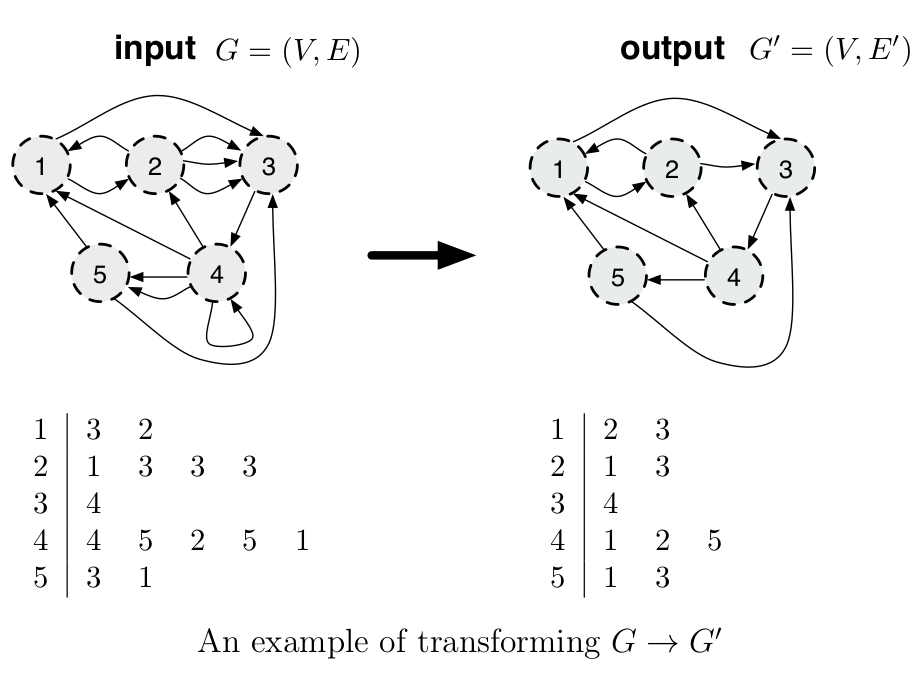
\includegraphics[width=1\textwidth]{P4}
\end{figure}

\textit{Describe and analyze an algorithm (explain how it works, give
  pseudocode if necessary, derive its running time and space usage,
  and prove its correctness) that takes $O(V + E)$ time and space to
  convert $G$ into $G'$, and thereby will solve any of the Sphinx’s
  questions. Assume both $G$ and $G'$ are stored as adjacency lists.}

\textit{Hermione’s hints: Don’t assume adjacencies \texttt{Adj[u]} are
  ordered in any particular way, and remember that you can add edges
  to the list and then remove ones you don't need.}
\\\\
Here's a complete algorithm in python3:\\
\textit{let g = 2 dimensional list representing the adjacency lists.\\ Verticies are numbered starting at 0}\\
\begin{verbatim}
def convert(g):
  for i in range(len(g)):
    j = 0
    t = {i:1}
    while j < len(g[i]):
      if g[i][j] in t:
        g[i].pop(j)
      else: 
        t[g[i][j]] = 1
        j += 1
\end{verbatim}

This algorithm works by scanning through all adjacency lists $u$.adj $\forall$ $u$ $\in$ V, and deleting all duplicate verticies (multipaths) as well as occurances of $u$ (self-loops). Duplicates are kept track of using a hashmap (dictionary in the above Python), thus determining if a vertex has been seen before is $\Theta(1)$. 

\textbf{Time - }The outer loop runs $|V| = n$ times, and the inner loop will run $\sum_{i=0}^{n}{V[i].adj.length}$ = $|E|$ times. Because each operation inside the inner loop is constant, the total running time is $O(V + E)$ 

\textbf{Space - }The only auxiliary space needed is the hashmap which takes $O(V)$ space (For each vertex, there can be at most one edge between each vertex)
\pagebreak

\textbf{Correctness:} Consider the inner loop, which is run for each vertex $u$ $\in V$:

\textit{Invariant: } g[i][0 .. j-1] = \{g[i][0 .. j-1]\} $\wedge$ i $\notin$ g[i][0 .. j-1] (i.e. $V_i$.adj contains no duplicates or $V_i$)

\textit{Initialization: } Before the loop enters, j=0 $\implies$ g[0][0..j-1] = $\O$ = \{$\O$\}, i $\notin$ $\O$

\textit{Maintainence: } During the loop, if g[i][j] is in the map of values we have seen before then it is deleted from g[i]. Because i was previously inserted into the map, every occurance of i will be deleted. If if g[i][j] is not in the map, it is added to the map, and j is increased. Note that j does not need to be increased if we delete a value, because the length of g[i] shrinks by 1, which has the same effect. After this, j-1 is the index of the vertex we just evaluated -- in the event we deleted it, the invariant still holds as it is no longer in g[i], in the event we didn't, it was the first value of j seen so it was added to the map and the variant still holds. 

\textit{Termination: } After the loop exits, j = g[i].length $\implies$ g[i][0 .. j-1] = g[i] = \{g[i]\} as every duplicate vertex and vertex = i was removed. 

\newpage


% ******************* PROBLEM 5 *********************
\section*{Problem 5}

\textit{(15 pts extra credit) Professor McGonagall has provided the
  young wizard Ron with three magical batteries whose sizes are 42,
  27, and 16 morts, respectively. (A mort is a unit of wizard energy.)
  The 27-mort and 16-mort batteries are fully charged (containing 27
  and 16 morts of energy, respectively), while the 42-mort battery is
  empty, with 0 morts. McGonagall says that Ron is only allowed to
  use, repeatedly, if necessary, the \textbf{mort transfer spell} when
  working with these batteries. This spell transfers all the morts in
  one battery to another battery, and it halts the transfer either
  when the source battery has no morts remaining or when the
  destination battery is fully charged (whichever comes first).}

\textit{McGonagall challenges Ron to determine whether there exists a
  sequence of mort-transfer spells that leaves exactly 12 morts either
  in the 27-mort or in the 16-mort battery.}

\begin{enumerate}
\item[(a)]{\textit{Ron knows this is actually a graph problem. Give a
      precise definition of how to model this problem as a graph, and
      state the specific question about this graph that must be
      answered.}}
  \\\\
  Let each vertex be a 3-tuple value in the form a/b/c where a = level of the 27-mort battery, b = level of the 16-mort battery, and c = level of the 42-mort battery. \\
  A graph can be made of the possible states that can be obtained by one of the possible set of arguments to the mort transfer spell: $mts(a,b), mts(a,c), ... , mts(c,b)$: \\
  \includegraphics[width=10cm,height=8cm]{5-G}

  Each edge is bidirectional unless illustrated with an arrow indicating direction. 
  \pagebreak
\item[(b)]{\textit{What algorithm should Ron apply to solve the graph
      problem?}}
  \\\\
  Dijkstra
  \\
\item[(c)]{\textit{Apply that algorithm to McGonagall’s
      question. Report and justify your answer.}}
  \\\\
(27,16,0) \\
$ mts(a,c) \Rightarrow$ (0,16,27) \\
$ mts(b,c) \Rightarrow$ (0,1,42) \\
$ mts(c,a) \Rightarrow$ (27,1,15) \\
$ mts(a,b) \Rightarrow$ (12,16,15)

\end{enumerate}
  
% ---------------------------------------------------
  \newpage

\textbf{References} \\
\hrulefill
\begin{enumerate}
  \item CLRS
\end{enumerate}
\end{document}